\documentclass[mathserif]{beamer}

\usepackage{thesis}
\usepackage{pdfpages}
\usepackage{array}
\usepackage{booktabs}


\title[Sampling from Probabilistic Submodular Models]
{Sampling from Probabilistic Submodular Models}

\author[Alkis Gotovos]{}


\newcommand{\tab}[2]{%
\makebox[#1\linewidth][l]{#2}%
}

\begin{document}

\setbeamertemplate{background canvas}{}
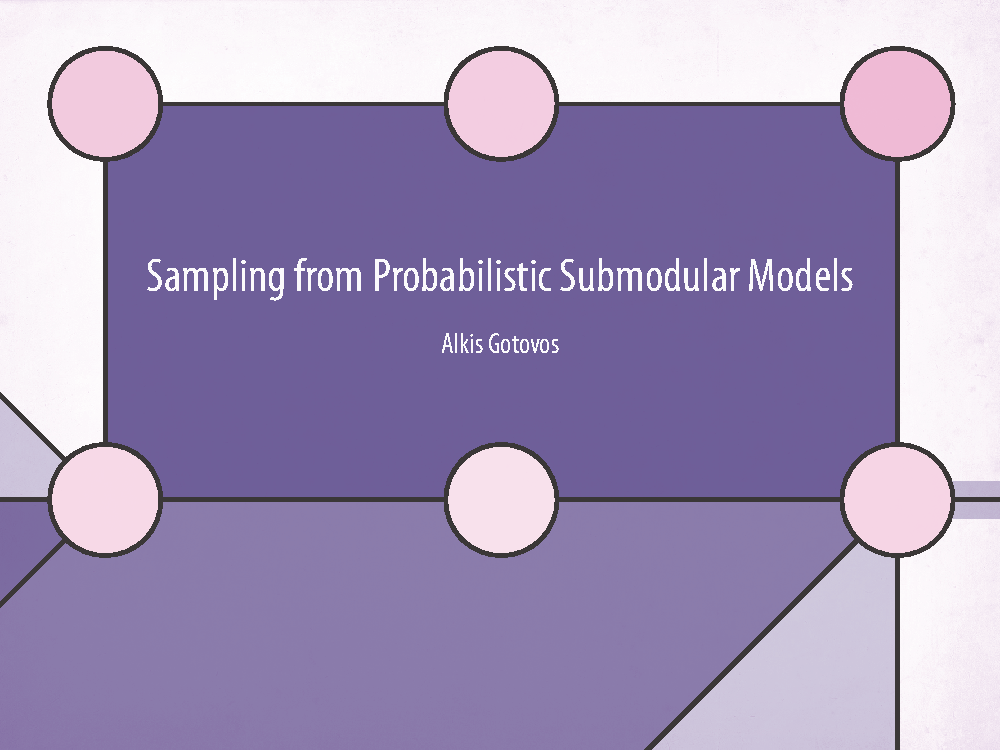
\includepdf[pages={1}]{title/title.pdf}
\setbeamertemplate{background canvas}{
\includegraphics[width=\paperwidth]{figures/bg_no_line.png}}


\begin{frame}{The Cancer Genome Atlas}
\vspace{0.5em}
\centering
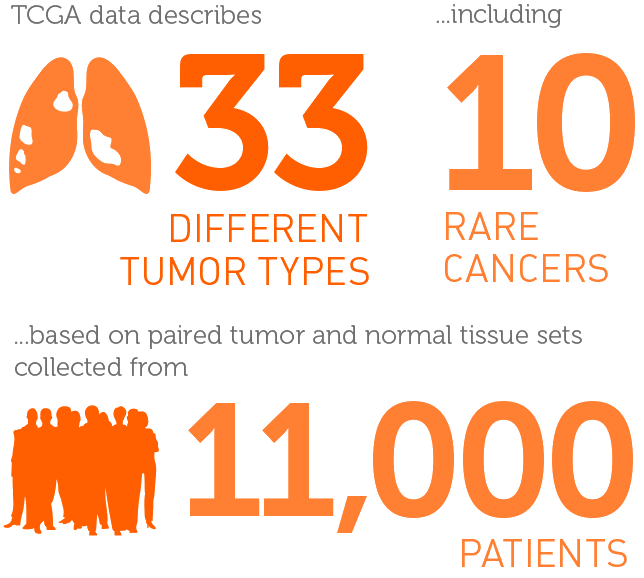
\includegraphics[width=2.5in]{figures/tcga.png}\\[-0.3em]
\hspace{12em}\qsource{cancergenome.nih.gov}
\end{frame}

\begin{frame}{The Cancer Genome Atlas}
\vspace{0.3em}
\centering
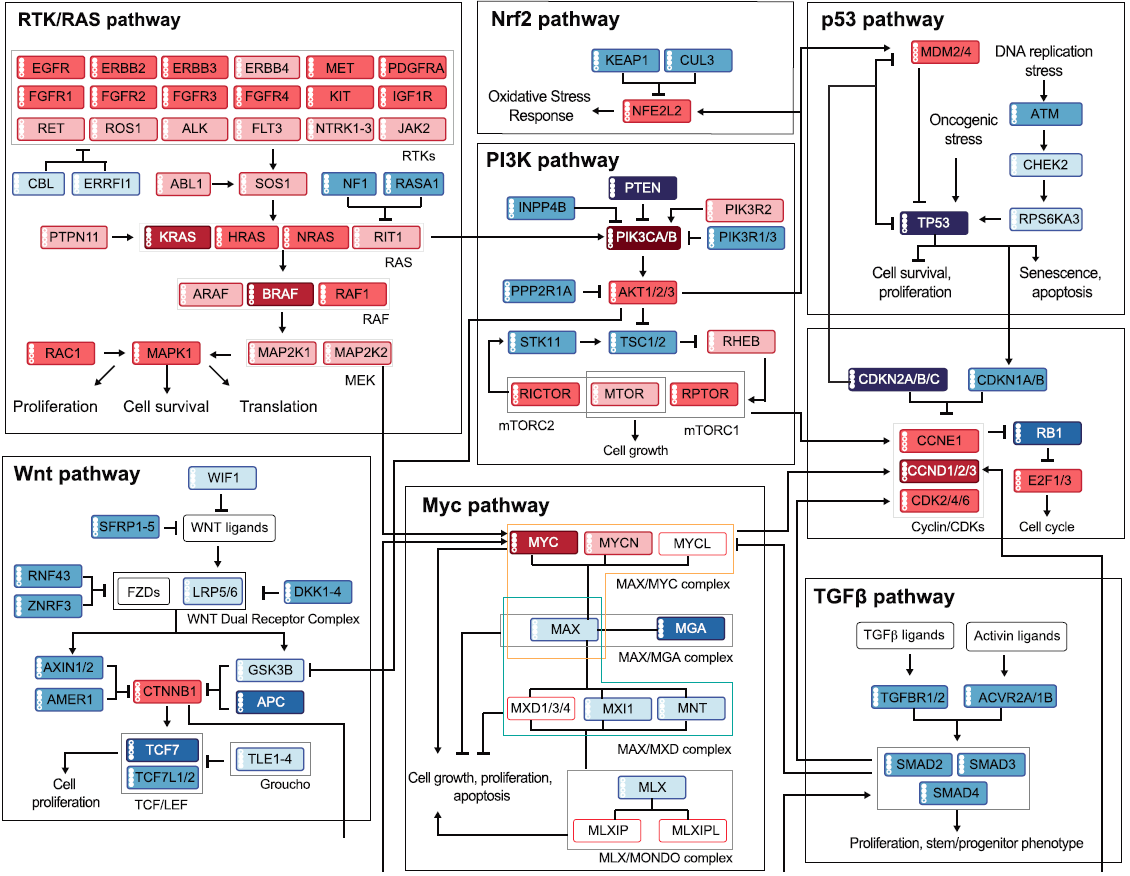
\includegraphics[width=3.85in]{figures/pathways_new.png}\\[-0.7em]
\hspace{22em}\qsource{Schultz et al., 2018}
\end{frame}

\begin{frame}{Modeling Interactions between Gene Mutations}
\centering
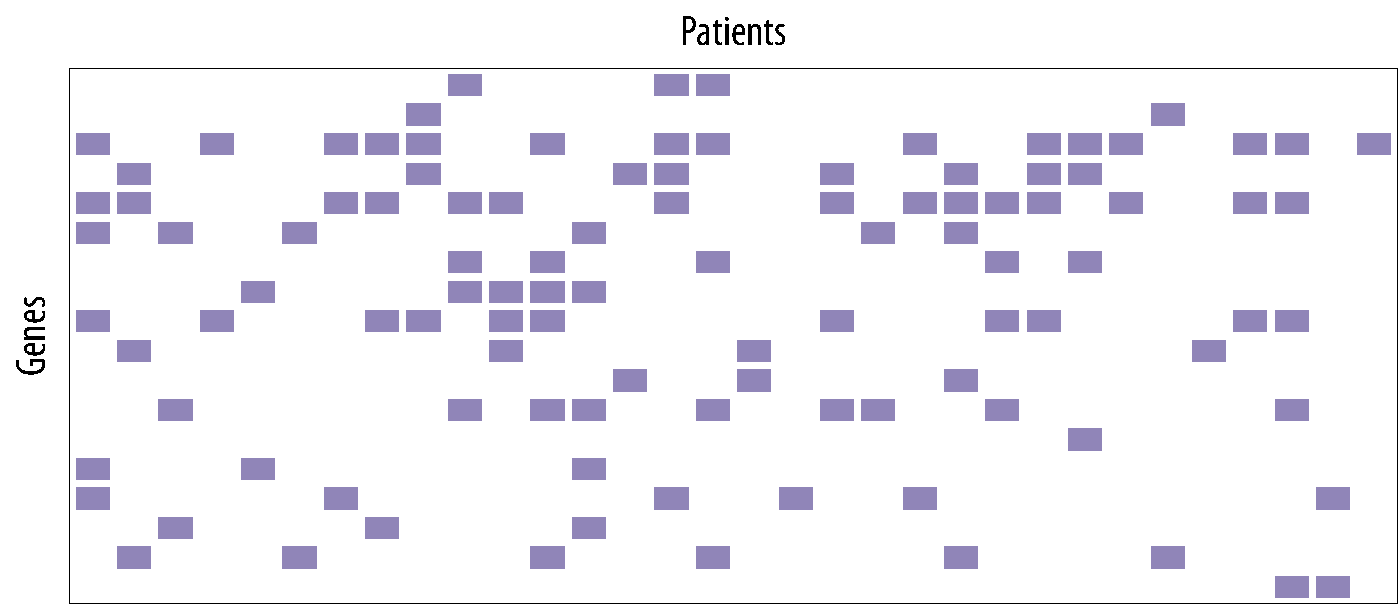
\includegraphics[width=3.7in]{figures/example1.pdf}
\end{frame}

\begin{frame}{Modeling Interactions between Gene Mutations}
\centering
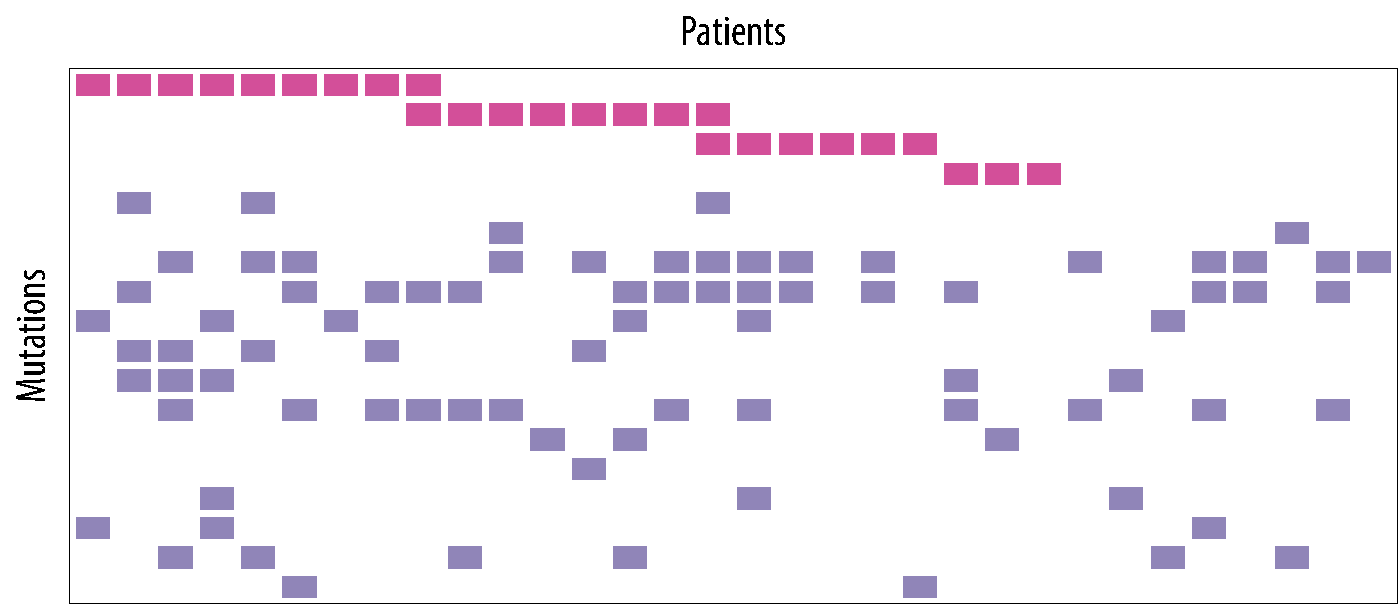
\includegraphics[width=3.7in]{figures/example1_rep.pdf}
\end{frame}

\begin{frame}{Modeling Interactions between Gene Mutations}
\centering
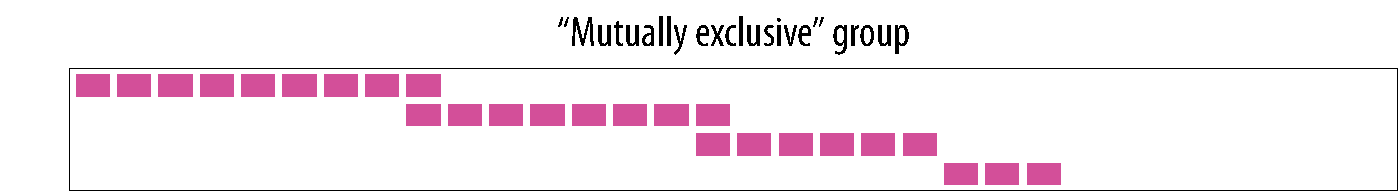
\includegraphics[width=3.7in]{figures/example1_rep_group.pdf}

\vspace{3em}

\begin{itemize}
\item<2-> \tab{0.4}{Discrete optimization \hspace{0.3em} 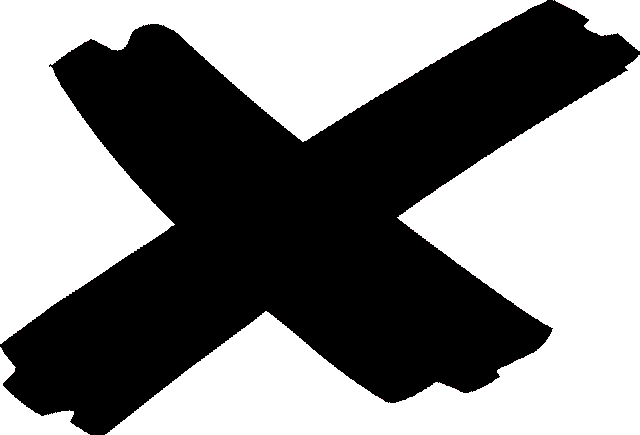
\includegraphics[width=0.13in]{figures/cross_mark.png}} \tab{0.15}{$\longrightarrow$} probabilistic models \hspace{0.3em} 
\includegraphics[width=0.13in]{figures/check_mark.png}
\vspace{0.7em}
\item<3-> \tab{0.4}{Classic pairwise models \hspace{0.3em} 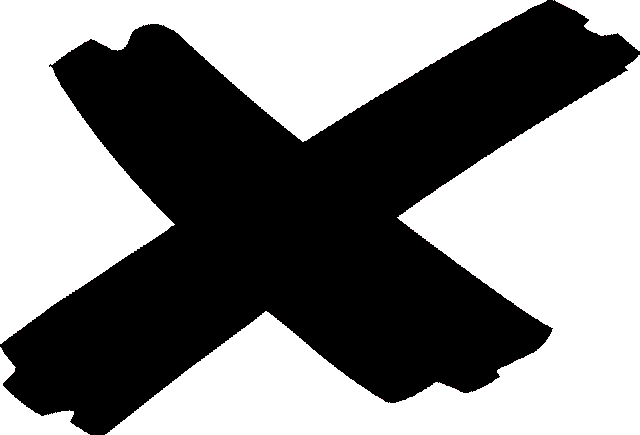
\includegraphics[width=0.13in]{figures/cross_mark.png}} \tab{0.15}{$\longrightarrow$} higher-order interactions \hspace{0.3em} 
\includegraphics[width=0.13in]{figures/check_mark.png}
\vspace{0.7em}
\item<4-> \tab{0.4}{Deep nets \hspace{0.3em} 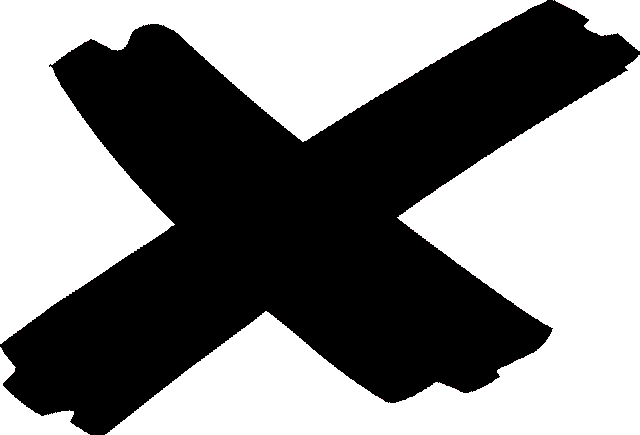
\includegraphics[width=0.13in]{figures/cross_mark.png}} \tab{0.15}{$\longrightarrow$} structured prior assumptions \hspace{0.3em} 
\includegraphics[width=0.13in]{figures/check_mark.png}
\end{itemize}
\end{frame}

\begin{frame}{Probabilistic Submodular Models}

\begin{center}
Distributions over subsets of $V = \{1,\ldots,n\}$

\vspace{0.8em}
\qboxa{
$p(S; \btheta) = \displaystyle\frac{1}{Z(\btheta)}\exp \big( F(S; \btheta) \big)$
}
\end{center}
\vspace{1.5em}

\begin{columns}
\begin{column}{0.54\textwidth}
\begin{itemize}
\item<2-> $F : 2^V \to \mathbb{R}\ $ is sub- or supermodular
\item<2-> $Z\ $ is the normalizer
\item<2-> $\btheta\ $ is a parameter vector
\end{itemize}
\vspace{0.6em}
\end{column}
\begin{column}{0.39\textwidth}
\uncover<3->{%
Well-studied subclasses
\begin{itemize}
\item Ising model (log-supermodular)
\item DPP (log-submodular)
\end{itemize}
}
\end{column}
\end{columns}

\end{frame}

\begin{frame}{Inference}
\vspace{1.75em}
\begin{center}
Distributions over subsets of $V = \{1,\ldots,n\}$

\vspace{0.8em}
\qboxa{
$p(S; \btheta) = \displaystyle\frac{1}{Z(\btheta)}\exp \big( F(S; \btheta) \big)$
}
\end{center}
\vspace{2em}

\uncover<2->{%
Fundamental tasks
}
\vspace{0.5em}
\hspace{11em}\tikzmark{right}
\begin{itemize}
\item<3-> Compute marginals $\ \mathbb{P}(a \in S \mid \{b, c\} \subseteq S)$ \tikzmark{i2}
\item<3-> Compute $\ Z$ \tikzmark{i3}
\item<5> Learn $\btheta$ from data
\end{itemize}

\uncover<4->{%
\begin{tikzpicture}[overlay, remember picture]
\node[anchor=base] (a) at (pic cs:i2) {\vphantom{h}}; % push the mark to the top of the line (ie including ascenders)
\node[anchor=base] (b) at (pic cs:i3) {\vphantom{g}}; % push the mark to the bottom of the line (ie including descenders)
\draw [decoration={brace,amplitude=0.5em},decorate,thick,col2]
 (a.north -| {pic cs:right}) -- (b.south -| {pic cs:right});
\node [text=col2,xshift=10.4em] (t) at ($(a)!0.5!(b)$) {\#P-hard in general};
\end{tikzpicture}
}

\end{frame}

\begin{frame}{Inference}
\vspace{0.5em}

\begin{minipage}{\textwidth}
\begin{columns}[c]
\column{0.36\textwidth}
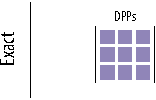
\includegraphics[height=0.7in]{figures/inf_dpp.pdf}
\column{0.57\textwidth}
\begin{itemize}
\item Tractable only for limited subclasses
\vspace{0.3em}
\item \#P-hard even for Ising models
\end{itemize}
\end{columns}
\end{minipage}

\uncover<2->{%
\vspace{2em}
\begin{minipage}{\textwidth}
\begin{columns}[c]
\column{0.36\textwidth}
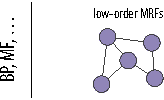
\includegraphics[height=0.7in]{figures/inf_mrf.pdf}
\column{0.57\textwidth}
\begin{itemize}
\item Extensively studied model class
\vspace{0.3em}
\item Complexity exponential in model order
\end{itemize}
\end{columns}
\end{minipage}
}

\uncover<3->{%
\vspace{2em}
\begin{minipage}{\textwidth}
\begin{columns}[c]
\column{0.36\textwidth}
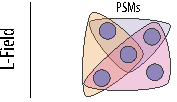
\includegraphics[height=0.7in]{figures/inf_psm.pdf}
\column{0.57\textwidth}
\begin{itemize}
\item Variational approach for general PSMs\\
\qcitea{Djolonga and Krause, 2014; Djolonga and Krause, 2015}
\end{itemize}
\end{columns}
\end{minipage}
}
\end{frame}

\begin{frame}{Thesis Topic}
\vspace{1em}
\centering
\only<1>{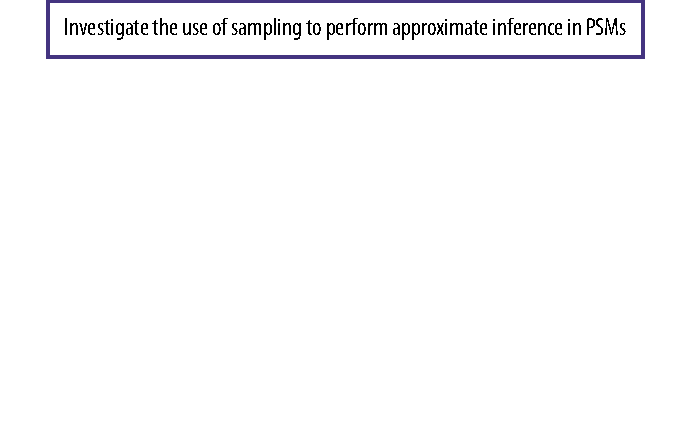
\includegraphics[width=\textwidth]{figures/chapters_topic.pdf}}%
\only<2>{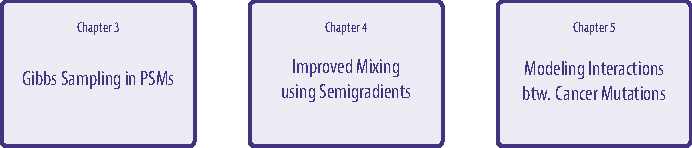
\includegraphics[width=\textwidth]{figures/chapters.pdf}}
\end{frame}

\begin{frame}{Publications}
\vspace{0.5em}
\small
\begin{itemize}
\item P. Wenk, A. Gotovos, S. Bauer, N. S. Gorbach, A. Krause, J. Buhmann. Fast Gaussian Process Based Gradient Matching for Parameter Identification in Systems of Nonlinear ODEs. \emph{AISTATS}, 2019.
\vspace{0.5em}
\item {\color{col1dark}A. Gotovos, H. Hassani, A. Krause, S. Jegelka. Discrete Sampling using Semigradient-based Product Mixtures. \emph{UAI}, 2018.}
\vspace{0.5em}
\item {\color{col1dark}A. Gotovos, H. Hassani, A. Krause. Sampling from Probabilistic Submodular Models. \emph{NIPS}, 2015.}
\vspace{0.5em}
\item Y. Sui, A. Gotovos, J. W. Burdick, A. Krause. Safe Exploration for Optimization with Gaussian Processes. \emph{ICML}, 2015.
\vspace{0.5em}
\item A. Gotovos, A. Karbasi, A. Krause. Non-monotone Adaptive Submodular Maximization. \emph{IJCAI}, 2015.
\vspace{0.5em}
\item L. Heng, A. Gotovos, A. Krause, M. Pollefeys. Efficient Visual Exploration and Coverage with a Micro Aerial Vehicle in Unknown Environments. \emph{ICRA}, 2015.
\vspace{0.5em}
\item G. Hitz, A. Gotovos, F. Pomerleau, M. E. Garneau, C. Pradalier, A. Krause, R. Siegwart. Fully Autonomous Focused Exploration for Robotic Environmental Monitoring. \emph{ICRA}, 2014.
\end{itemize}
\end{frame}

\begin{frame}{Gibbs Sampling in PSMs}
\vspace{1em}
\centering
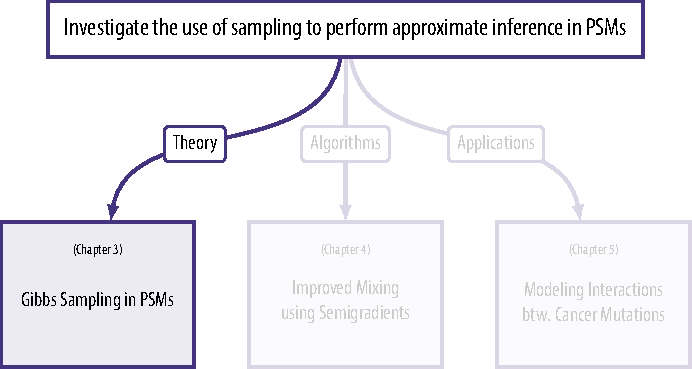
\includegraphics[width=\textwidth]{figures/chapters1.pdf}
\end{frame}

\begin{frame}{MCMC Sampling}
\begin{itemize}
\item Ground set $\ V = \{1,\ldots,n\}$
\item State space $\ \Omega = 2^V$
\item Transition matrix $\ P : \Omega \times \Omega \to \mathbb{R}$
\end{itemize}

%\vspace{1em}
\begin{center}
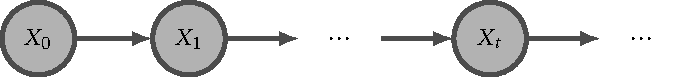
\includegraphics[width=3.3in]{figures/markov.pdf}
\end{center}

\vspace{1em}
\uncover<2->{%
Distance from stationarity $\ \ d(t) \defeq \max \left\{\|\mathbb{P}_{X_t} - p\|_{\textrm{tv}} \mid X_0 \in \Omega\right\}$}\\[1.5em]
\uncover<3->{Under mild conditions, $\ \ d(t) \xrightarrow{\ t\,\rightarrow\,\infty\ } 0\ \ \ \ $}\uncover<4->{{\color{col2} how fast?}}\\[1.6em]
\uncover<5->{Mixing time $\ \ t_{\textrm{mix}}(\epsilon) = \min \left\{t \mid d(t) \leq \epsilon \right\}$}
\end{frame}

\begin{frame}{The Gibbs Sampler}
\vspace{1em}
\centering
\only<1>{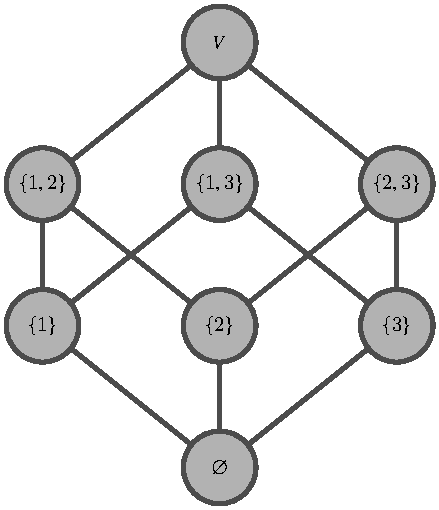
\includegraphics[width=2.5in]{figures/lattice_gibbs_0.pdf}}%
\only<2>{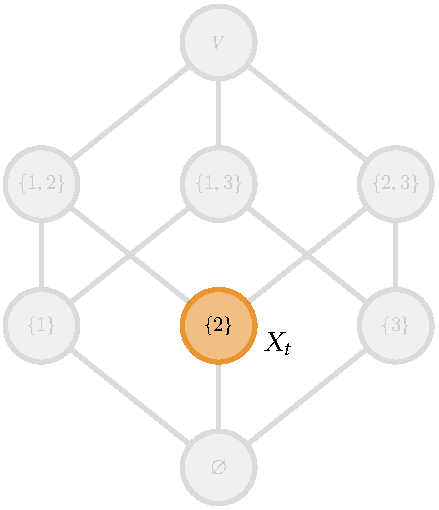
\includegraphics[width=2.5in]{figures/lattice_gibbs_1.pdf}}%
\only<3>{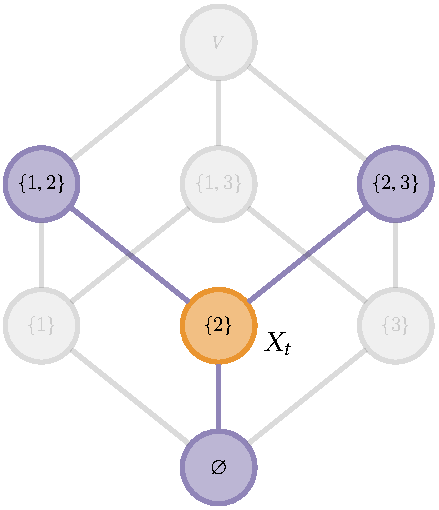
\includegraphics[width=2.5in]{figures/lattice_gibbs_2.pdf}}%
\end{frame}

\begin{frame}{The Gibbs Sampler}
\begin{center}
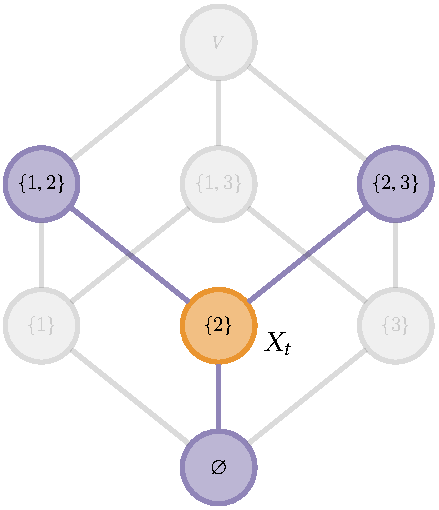
\includegraphics[width=1.4in]{figures/lattice_gibbs_2.pdf}
\end{center}

\centering
Mixing times are in general exponential in $|V|$ \qcitea{Jerrum and Sinclair, 1993}

\vspace{1em}
\centering
\qboxa{\minibox{We establish sufficient conditions for sub-exponential mixing\\of the Gibbs sampler on PSMs.}}
\end{frame}

\begin{frame}{Polynomial-time Mixing}
\vspace{0.5em}
\only<1>{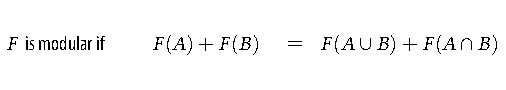
\includegraphics[width=3.9in]{figures/ineq_mod_0.pdf}}%
\only<2>{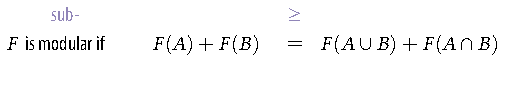
\includegraphics[width=3.9in]{figures/ineq_mod_1.pdf}}%
\only<3->{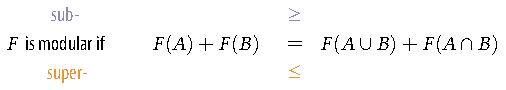
\includegraphics[width=3.9in]{figures/ineq_mod_2.pdf}}%

\uncover<4->{%
\vspace{1em}
``Distance" from modularity
\begin{align*}
\zeta_F \defeq \max_{A, B \subseteq V} \big|F(A) + F(B) - F(A \cup B) - F(A \cap B)\big|
\end{align*}
}

\uncover<5>{%
\qtheorem{1}{
For any sub- or supermodular set function $F$, the mixing time of the Gibbs sampler is
\begin{align*}
t_{\textrm{mix}}(\epsilon) = \mathcal{O}\left(n^2 \exp(\zeta_F)\log\epsilon^{-1}\right).
\end{align*}
}}
\end{frame}

\begin{frame}{Proof Outline}
\vspace{0.5em}
\only<1>{Need to route $p(S)p(R)$ amount of flow between each $S, R \subseteq V$\qcitea{Sinclair, 1992}}
\only<2-3>{Construct a ``canonical path'' between each $S, R \subseteq V$}
\only<4>{The Markov chain transition probabilities determine the edge capacities}
\only<5>{Congestion of an edge $\ \sim\ $ (total flow through edge) / capacity}
\only<6-7>{$t_{\mathrm{mix}}(\epsilon) = \mathcal{O}\left(\max\{\textrm{congestion}\}\log \epsilon^{-1}\right)$ \qcitea{Sinclair, 1992}}
\vspace{1em}

\only<1>{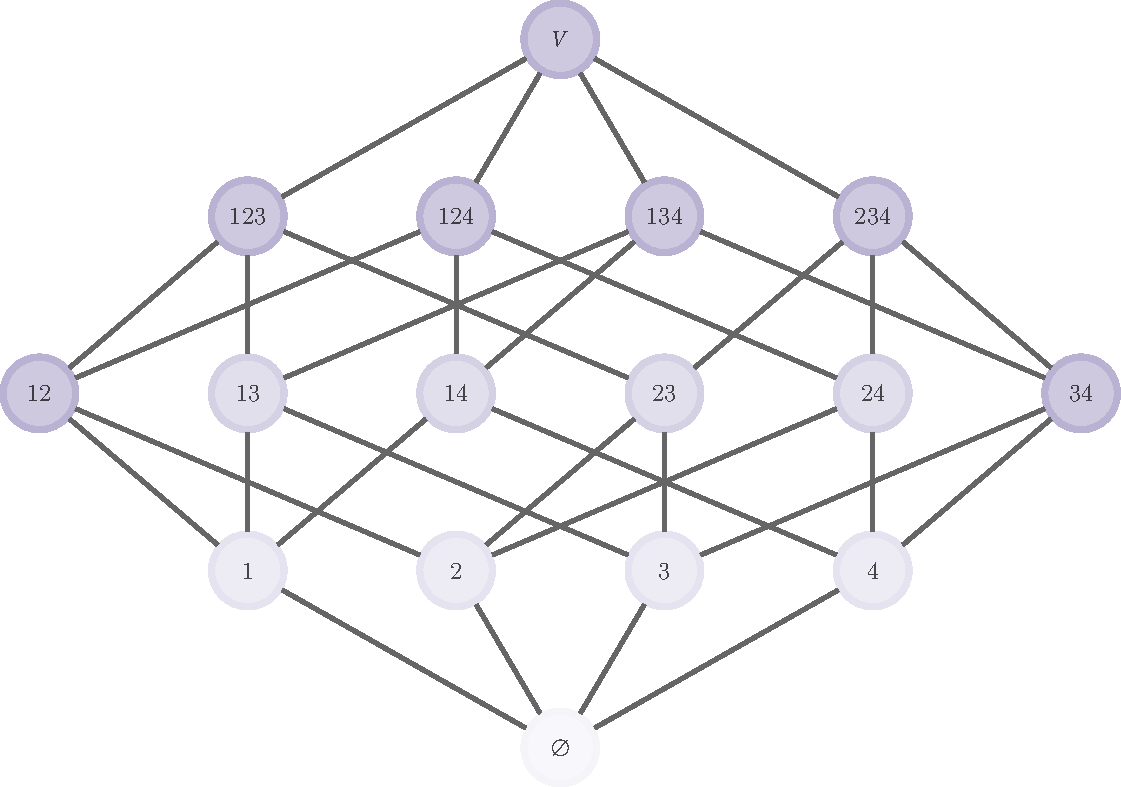
\includegraphics[width=0.9\textwidth]{figures/cp_easy.pdf}}%
\only<2>{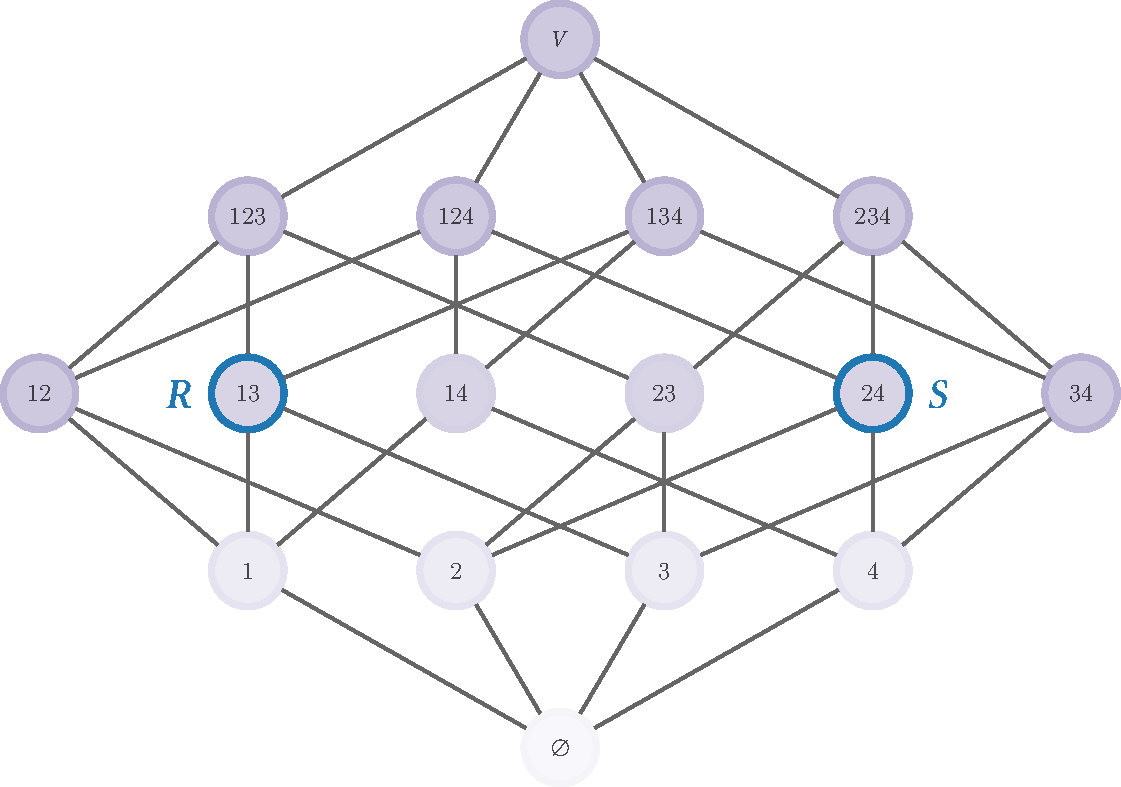
\includegraphics[width=0.9\textwidth]{figures/cp_easy_path_1.pdf}}%
\only<3>{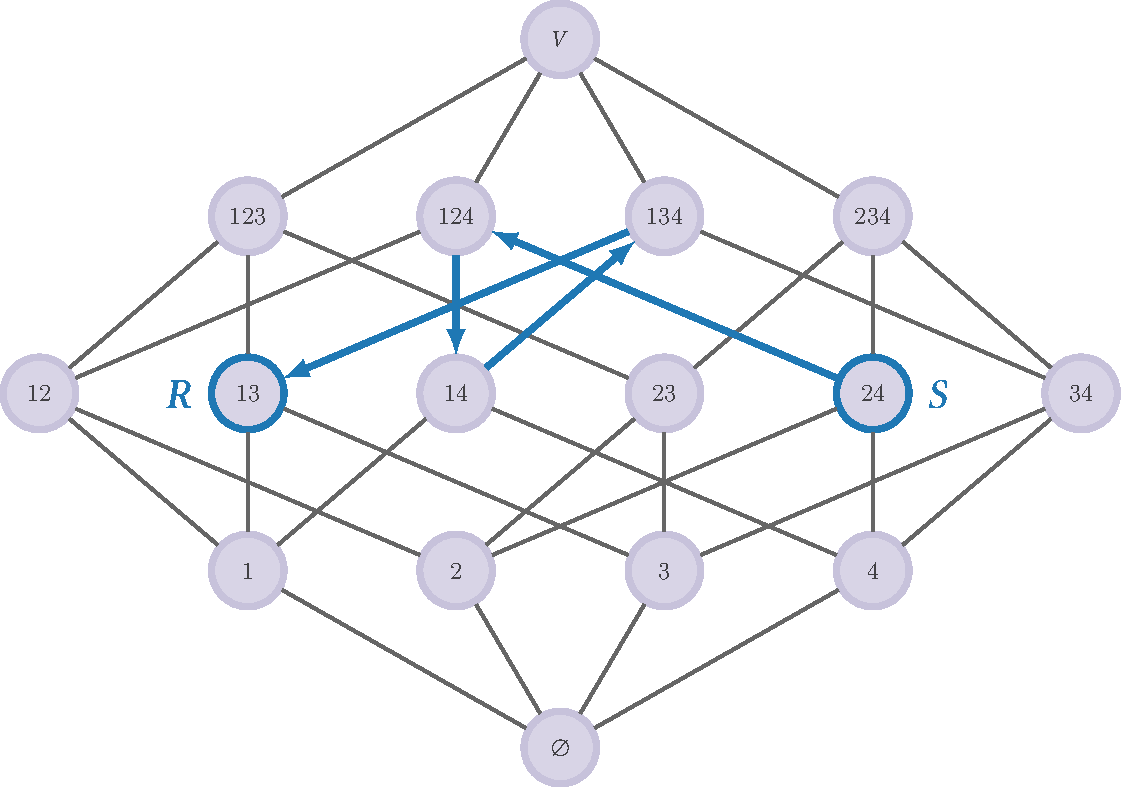
\includegraphics[width=0.9\textwidth]{figures/cp_easy_path_4.pdf}}%
\only<4>{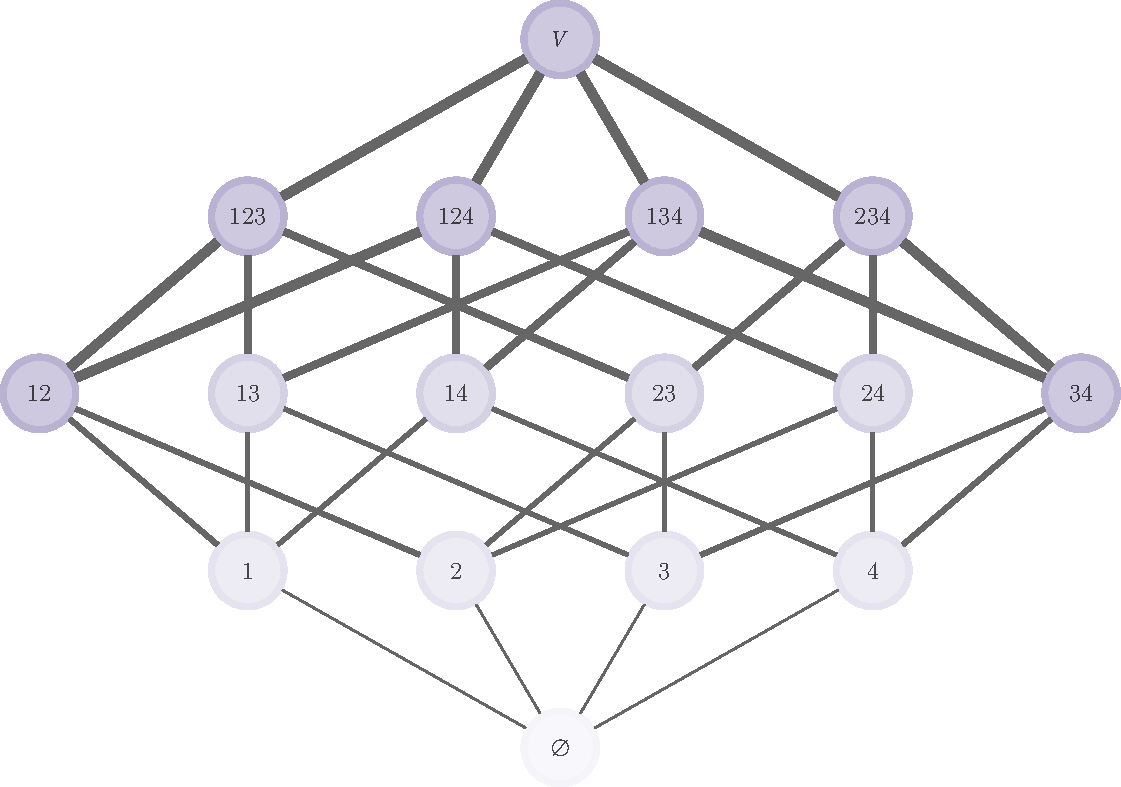
\includegraphics[width=0.9\textwidth]{figures/cp_easy_cap.pdf}}%
\only<5-6>{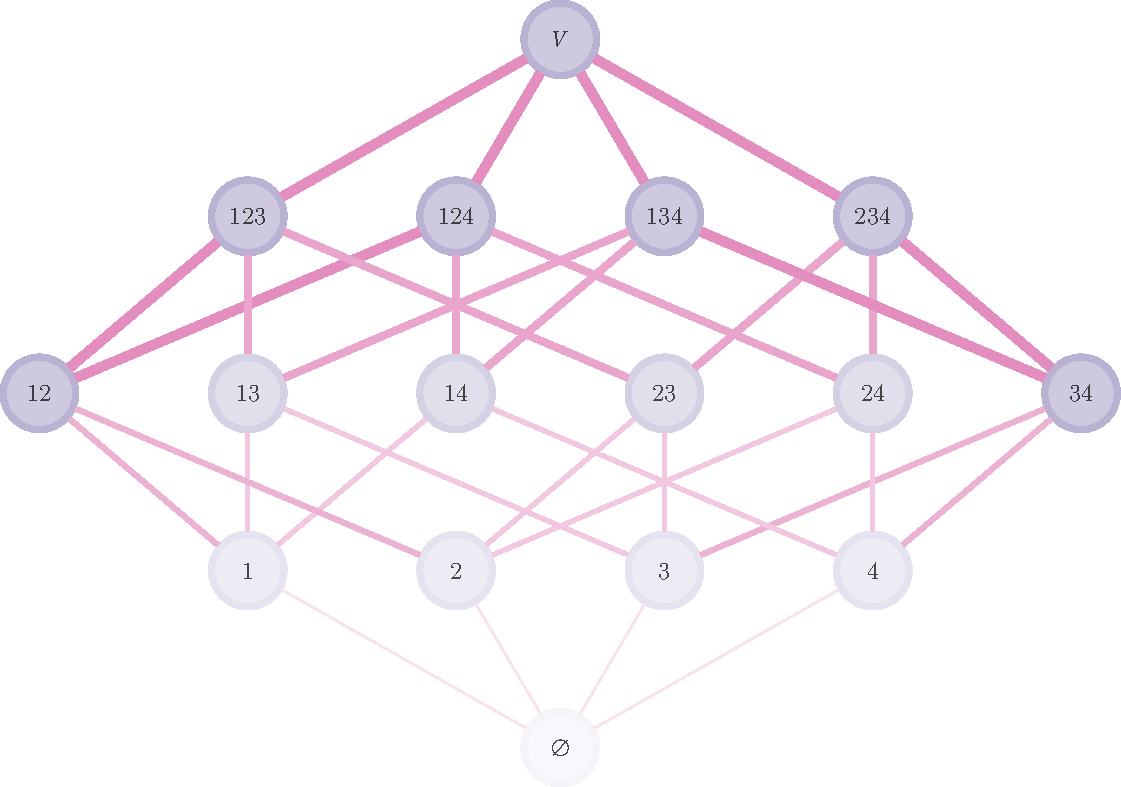
\includegraphics[width=0.9\textwidth]{figures/cp_easy_cong.pdf}}%
\only<7>{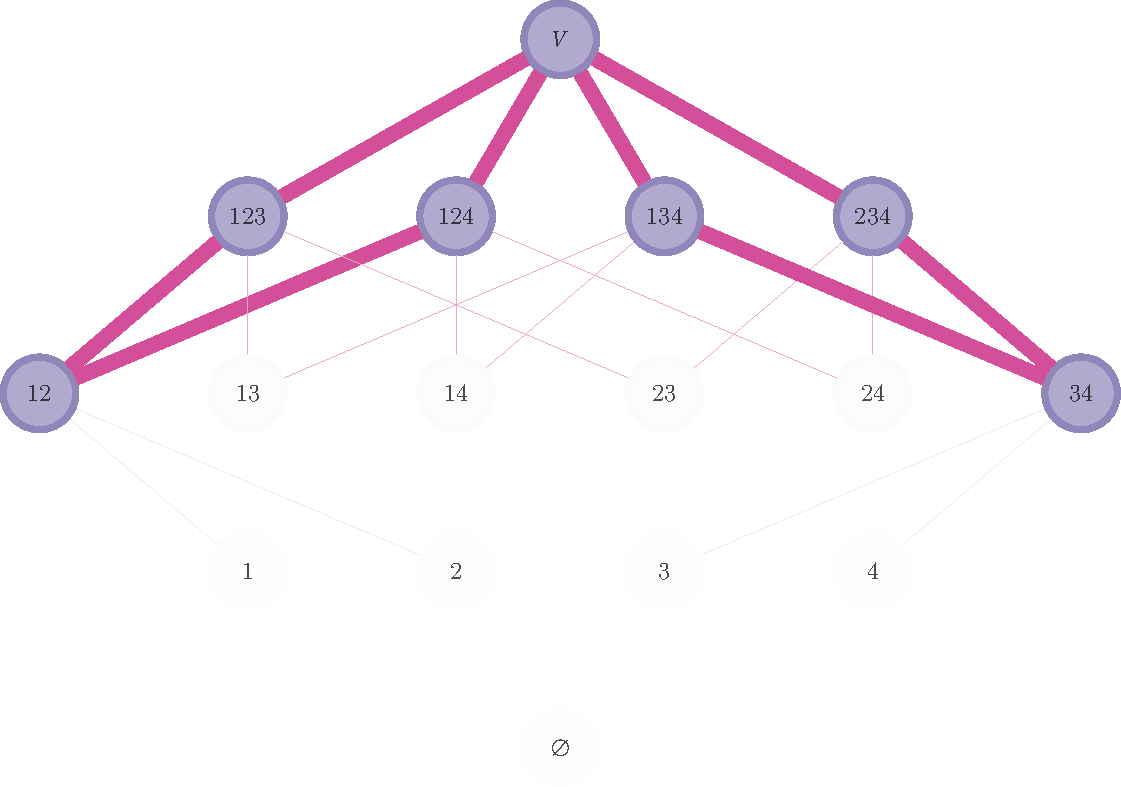
\includegraphics[width=0.9\textwidth]{figures/cp_hard_cong.pdf}}%
\end{frame}

\begin{frame}{Improved Mixing using Semigradients}
\centering
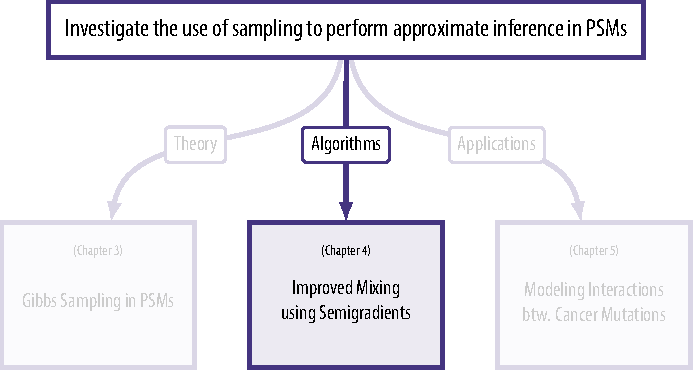
\includegraphics[width=\textwidth]{figures/chapters2.pdf}
\end{frame}

\begin{frame}{Bottlenecks}
\vspace{1em}
\centering
\only<1>{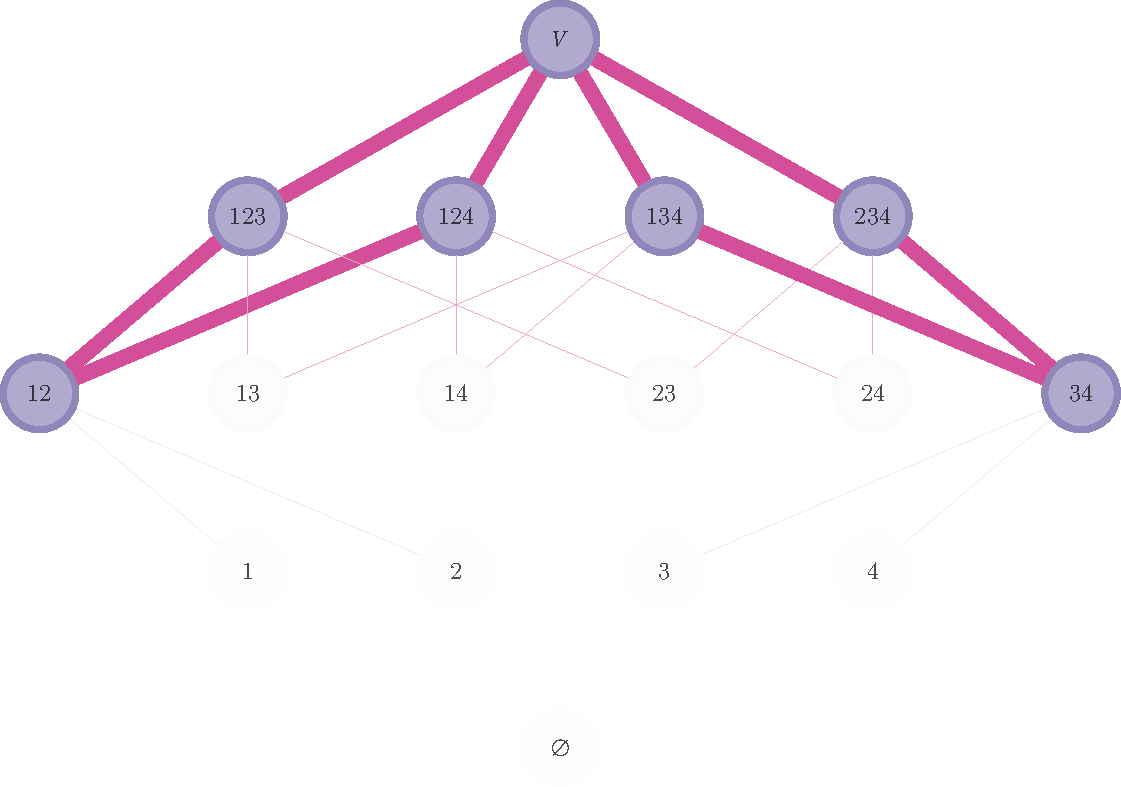
\includegraphics[width=0.9\textwidth]{figures/cp_hard_cong.pdf}}%
\only<2>{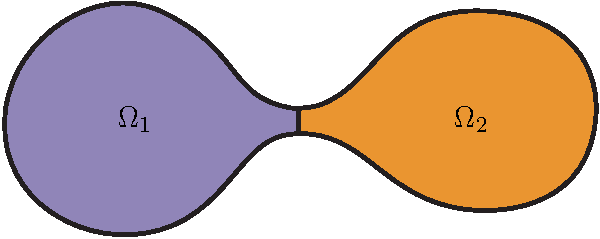
\includegraphics[width=0.9\textwidth]{figures/bottleneck1.pdf}}%
\only<3>{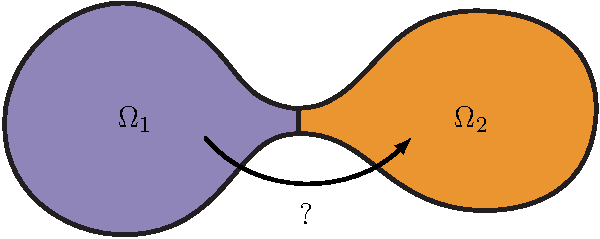
\includegraphics[width=0.9\textwidth]{figures/bottleneck2.pdf}}%
\end{frame}


\newcommand*\circled[1]{\tikz[baseline=-0.3ex,anchor=base]{\node[shape=circle,draw,inner sep=1.5pt] (char) {\scriptsize #1};}}
\begin{frame}{The \Ms{} Chain}
\vspace{0.8em}
\hspace{3pt} \Ms{} = Mixture of Log-Modulars Metropolis

\vspace{-1em}
\uncover<2->{
\renewcommand{\arraystretch}{1}
\begin{tabular}{>{\arraybackslash}p{0.28\textwidth}>{\arraybackslash}p{0.71\textwidth}}

\begin{minipage}[t]{\textwidth}
\vspace{1.8em}
\only<7-8>{\color{col2}} \circled{1}\hspace{0.3em} Mixture
\end{minipage}
&
\begin{minipage}[t]{\textwidth}
\uncover<8->{%
\vspace{1em}
\only<1-10>{$q(S, T) = \displaystyle\frac{1}{Z_q} \sum_{i = 1}^{r} w_i\exp\left(m_i(T) \right)$}%
\only<11->{${\color{col2}q(T)} = \displaystyle\frac{1}{Z_q} \sum_{i = 1}^{r} w_i\exp\left(m_i(T) \right)$}
\vspace{1em}%
}
\end{minipage}
\\ \midrule

\begin{minipage}[t]{\textwidth}
\vspace{1.15em}
\only<9-10>{\color{col2}} \circled{2}\hspace{0.3em} Log-Modulars
\end{minipage}
&
\begin{minipage}[t]{\textwidth}
\uncover<10->{
\vspace{1em}
$m_i(T) = \displaystyle\sum_{v \in T} m_{iv}$
\vspace{1em}
}
\end{minipage}
\\ \midrule

\begin{minipage}[t]{\textwidth}
\vspace{2.45em}
\only<3-6>{\color{col2}} \circled{3}\hspace{0.3em} Metropolis
\end{minipage}
&
\begin{minipage}[t]{\textwidth}
\vspace{1em}
\begin{itemize}
\item<4-> Target $\ p(S) \propto \exp(F(S))$
\vspace{0.15em}
\item<5-> \only<5-10>{Proposal $\ q(S, T)$}%
\only<11->{Proposal \color{col2} $\ q(T)$}%
\item<6-> Accept with probability%
\only<6-10>{$\ \ \min\left\{1, \frac{p(T)q(T, S)}{p(S)q(S, T)}\right\}$}%
\only<11->{$\ \ \min\left\{1, \frac{p(T)\color{col2}q(S)}{p(S)\color{col2}q(T)}\right\}$}%
\end{itemize}
\vspace{1em}
\end{minipage}

\end{tabular}
}
\end{frame}

\begin{frame}{The Combined Chain}
\vspace{0.5em}
Gibbs step with prob. $\delta$ \hspace{1em}|\hspace{1em} \Ms{} step with prob. $1 - \delta$

\uncover<2->{%
\vspace{2em}
\centering
\only<1-2>{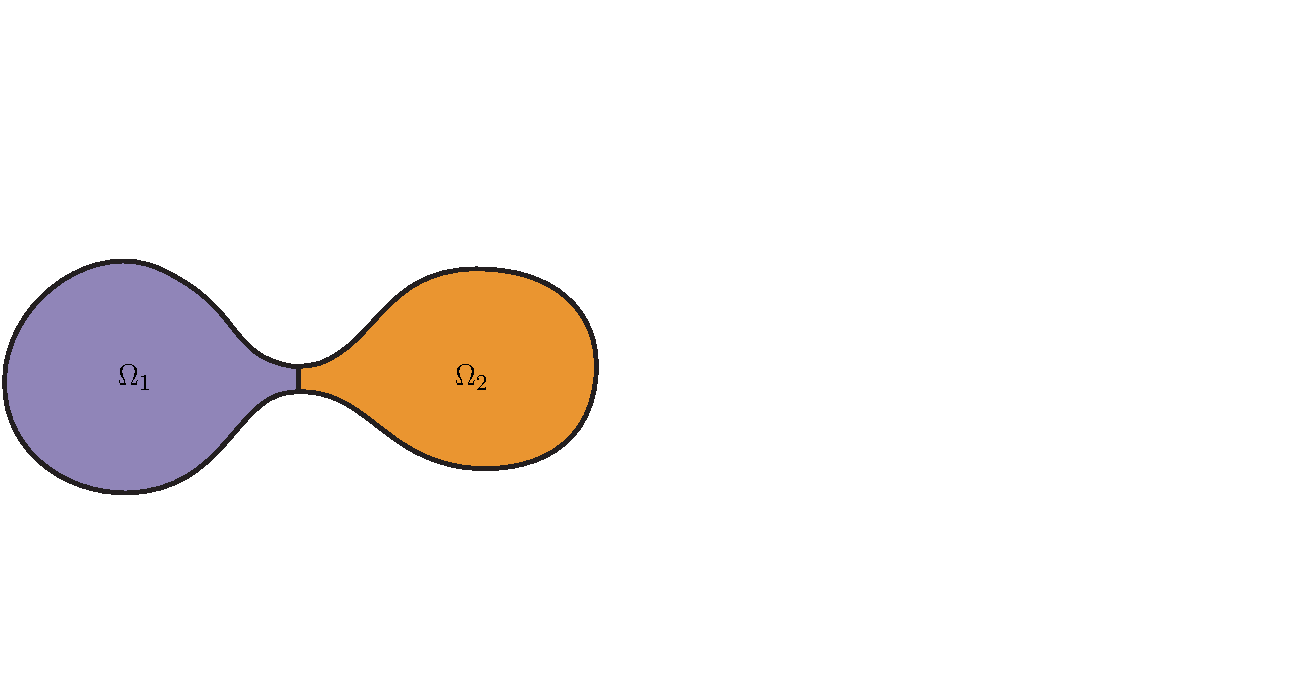
\includegraphics[width=\textwidth]{figures/decomposition1.pdf}}%
\only<3>{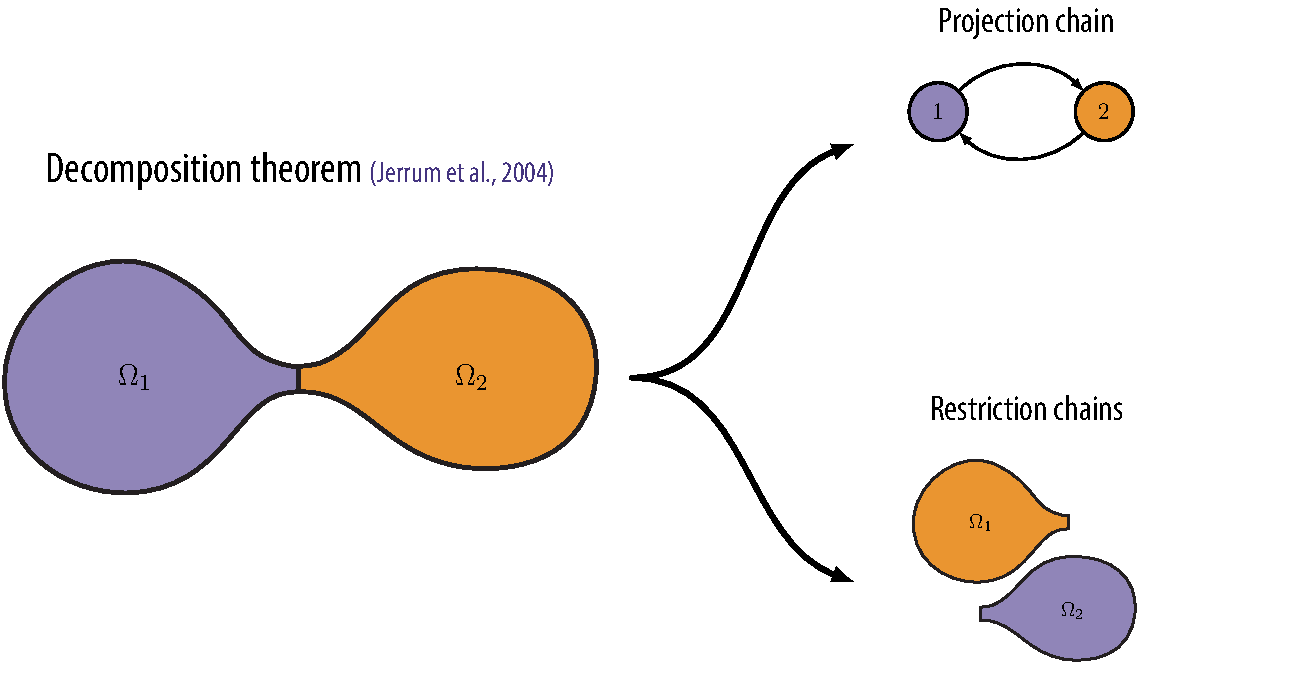
\includegraphics[width=\textwidth]{figures/decomposition2.pdf}}%
\only<4>{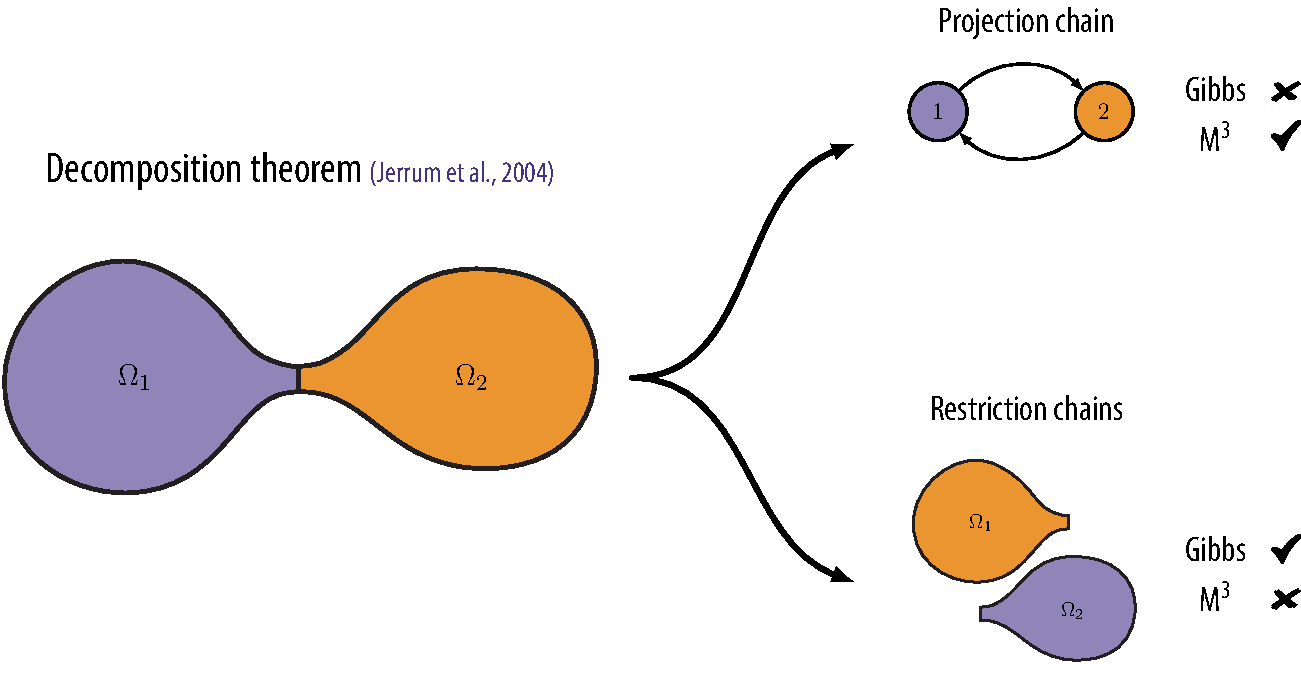
\includegraphics[width=\textwidth]{figures/decomposition.pdf}}%
}
\end{frame}

\begin{frame}{Constructing the Mixture}
\vspace{0.5em}
\only<1-3>{Construction}\only<4->{{\color{col1dark}Iterative} construction} of $\ q(\cdot) \propto \displaystyle\sum_{i = 1}^{r} \exp\left(m_i(\cdot) \right)$

\uncover<2->{%
\vspace{3em}
\begin{algorithmic}
  \REQUIRE Set function $F$, mixture size $r$
  \vspace{0.5em}
  \FOR{$i = 1$ \TO $r$}
  \vspace{0.3em}
  \LET{$\sigma$}{\only<1-3>{Permutation of $V$}\only<4->{{\color{col1dark}\textsc{Greedy}$\left(F(\cdot) - \log\displaystyle\sum_{j = 1}^{i-1} \exp(m_j(\cdot))\right)$}}}
  \vspace{0.3em}
  \LET{$m_i$}{\only<1-2>{Modular function that approximates $F$ at $\sigma$}\only<3->{\color{col2}\textsc{SemiGradient}$\left(F, \sigma\right)$}}%\only<4->{\textsc{SemiGradient}($F$, $\sigma$)}}
  \vspace{0.3em}
  \ENDFOR
  \RETURN $\{m_1, \ldots, m_r\}$
\end{algorithmic}%
}
\vspace{4em}
\end{frame}

\begin{frame}{Benefit of Combined Chain}
\vspace{1em}
\centering
\only<1>{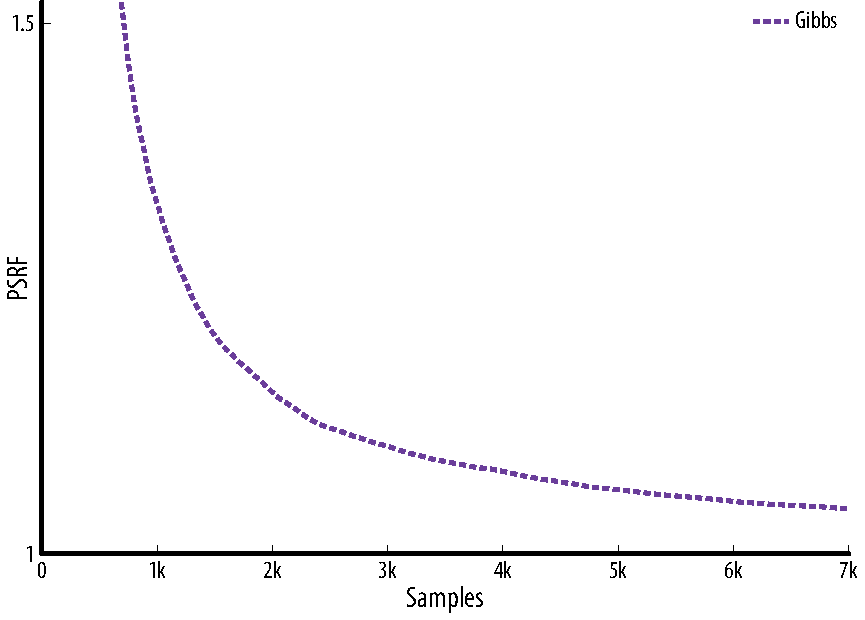
\includegraphics[width=\textwidth]{figures/exp3_1.pdf}}%
\only<2>{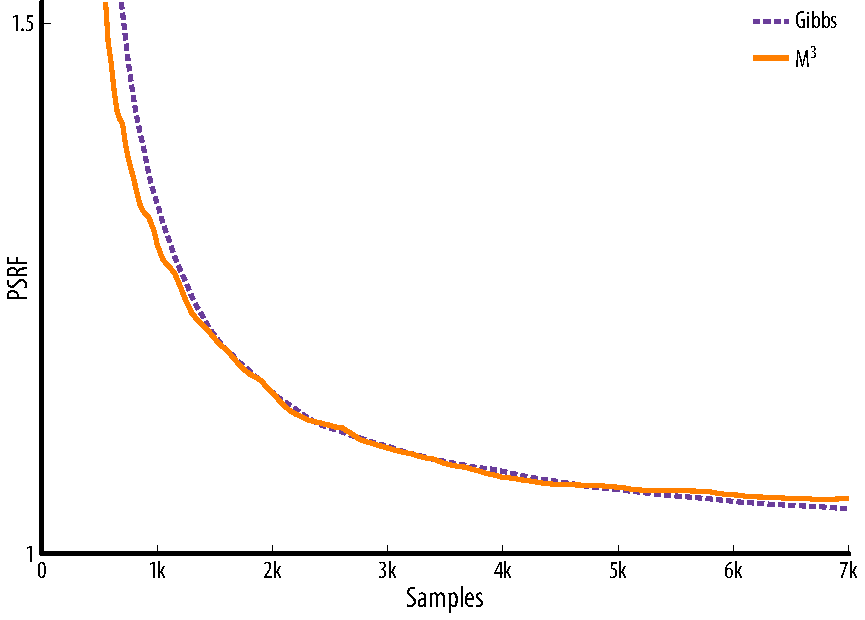
\includegraphics[width=\textwidth]{figures/exp3_2.pdf}}%
\only<3>{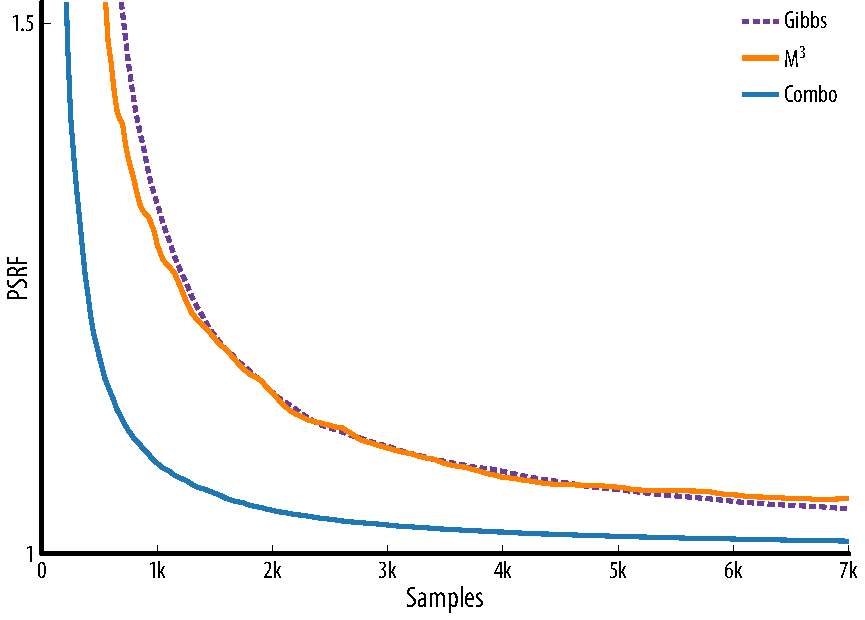
\includegraphics[width=\textwidth]{figures/exp3_3.pdf}}%
\end{frame}

\begin{frame}{Modeling Interactions between Cancer Mutations}
\centering
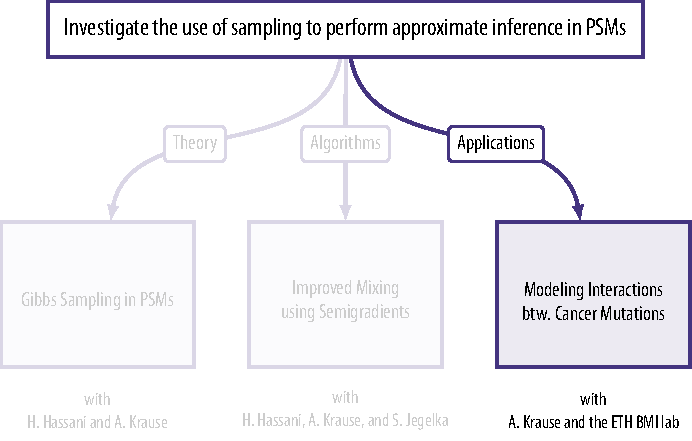
\includegraphics[width=\textwidth]{figures/chapters3.pdf}
\end{frame}

\begin{frame}{Approximate Maximum Likelihood Learning}
\vspace{-1em}
Data $\ \mathcal{D} = \{D_1,\ldots, D_N\}$

\uncover<2->{%
\only<1-2>{%
\vspace{3em}
\centering
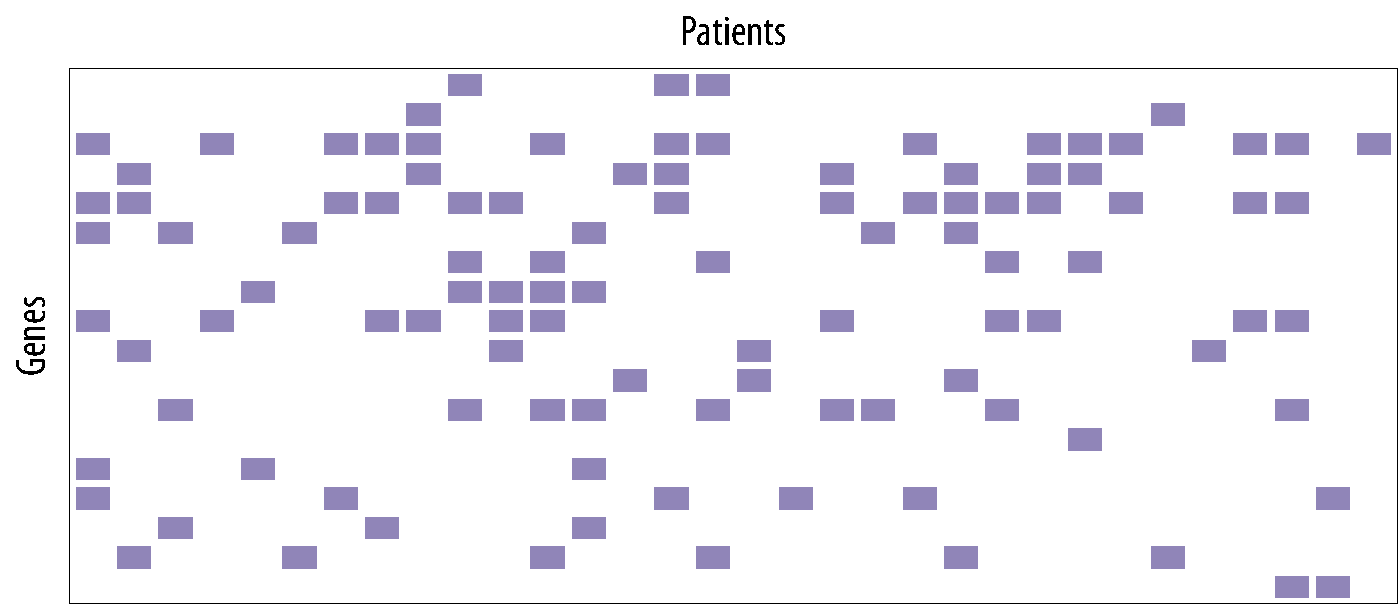
\includegraphics[width=3.7in]{figures/example1.pdf}
}%
\only<3->{%
\begin{align*}
\ell(\btheta) &= \sum_{i=1}^N F(D_i; \btheta) - N \log Z(\btheta)\\[1em]
\uncover<4->{\nabla_{\btheta} \ell(\btheta) &= \frac{1}{N}\sum_{i=1}^N \nabla_{\btheta} F(D_i; \btheta) - \alt<4>{}{\color{col2}}\mathbb{E}_{p}\left[ \nabla_{\btheta} F(S; \btheta)\right]\\[0.5em]}
\uncover<6->{&\approx \frac{1}{N}\sum_{i=1}^N \nabla_{\btheta} F(D_i; \btheta) - \color{col2}\frac{1}{M}\sum_{i=1}^M \nabla_{\btheta} F(S_i; \btheta)}
\end{align*}
}%
}
\end{frame}

\begin{frame}{The FLiD Model \qcitea{Tschiatscheck et al., 2016}}
\centering
\only<1>{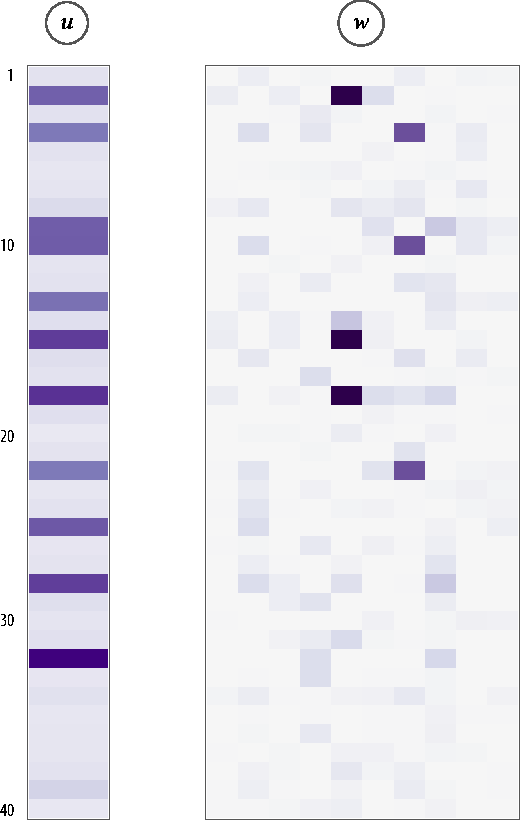
\includegraphics[height=0.9\textheight]{figures/mat_syn.pdf}}%
\only<2>{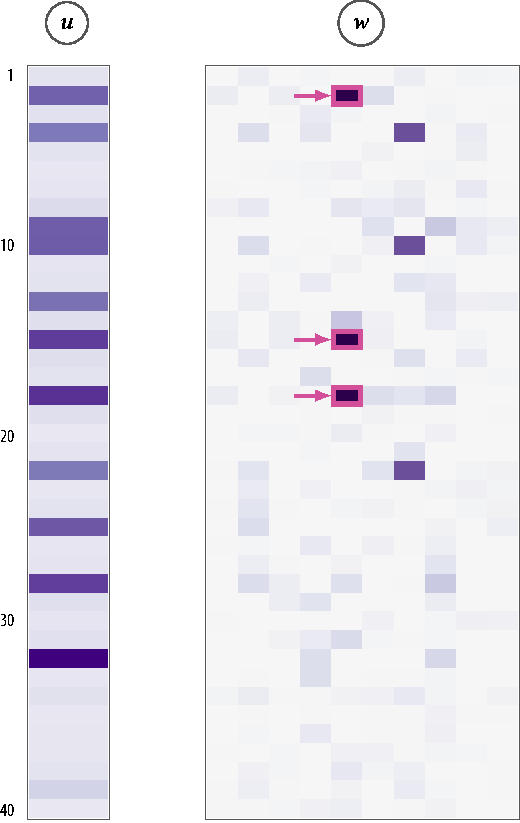
\includegraphics[height=0.9\textheight]{figures/mat_syn_1.pdf}}%
\only<3>{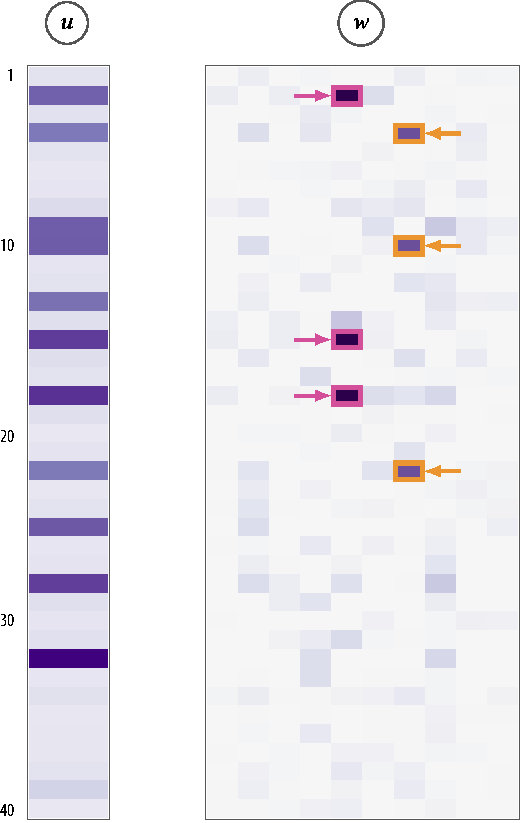
\includegraphics[height=0.9\textheight]{figures/mat_syn_2.pdf}}
\end{frame}

\begin{frame}{Synthetic Data}
$t\ $ groups of $k\ $ elements\\
\vspace{1em}
\centering
\only<1>{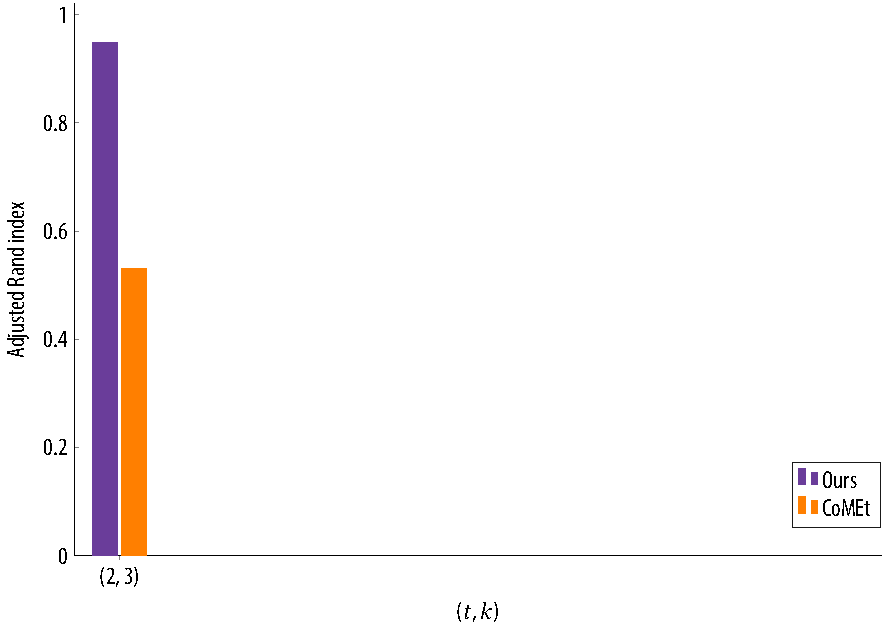
\includegraphics[width=0.93\textwidth]{figures/syn_multi_one.pdf}}%
\only<2>{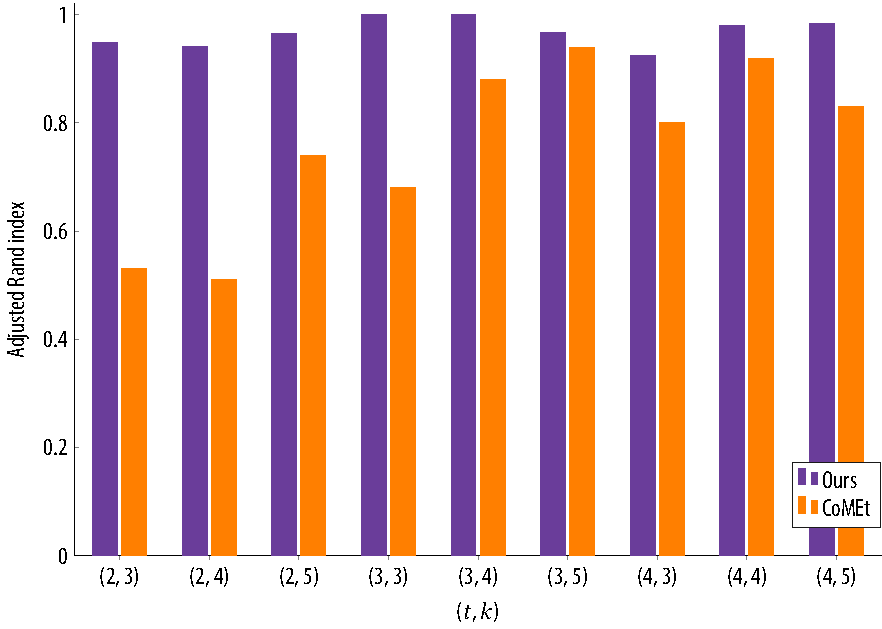
\includegraphics[width=0.93\textwidth]{figures/syn_multi.pdf}}%
\end{frame}

\begin{frame}{Real Cancer Data (TCGA AML)}
\vspace{1em}
\centering
\uncover<2->{\includegraphics[width=0.85\textwidth]{figures/aml_1.pdf}\\[2em]}
\uncover<3>{\includegraphics[width=0.85\textwidth]{figures/aml_3.pdf}}
\end{frame}

\begin{frame}{Real Cancer Data (TCGA AML)}
\vspace{1em}
\centering
\includegraphics[width=0.65\textwidth]{figures/graph_aml.pdf}
\end{frame}

\begin{frame}{Summary}
\vspace{1em}
\centering
\only<1>{\includegraphics[width=\textwidth]{figures/chapters_end_1.pdf}}%
\only<2>{\includegraphics[width=\textwidth]{figures/chapters_end_2.pdf}}%
\only<3>{\includegraphics[width=\textwidth]{figures/chapters_end_3.pdf}}%
\only<4>{\includegraphics[width=\textwidth]{figures/chapters_end.pdf}}%
\end{frame}

\end{document}
